\documentclass[prodmode,acmec]{ec-acmsmall}
\acmVolume{X}
\acmNumber{X}
\acmArticle{X}
\acmYear{2015}
\acmMonth{2}

\usepackage[english]{babel}
\usepackage[utf8]{inputenc}
\usepackage{amsmath}
\usepackage{subfigure}
\usepackage{floatrow}
\usepackage{hyperref}
%\usepackage{amsfonts}
%\usepackage{graphicx}

%\newtheorem{prop}{Proposition}
%\newtheorem{theorem}{Theorem}
%\newtheorem{definition}{Definition}
%\newtheorem{lemma}{Lemma}
%\newtheorem{cor}{Corollary}
\newtheorem{problem}{Problem}
%\newtheorem{conj}{Conjecture}

\bibliographystyle{acmsmall}

\begin{document}

\title{Information Monitoring in Routing Networks}
\author{David Burstein
\affil{University of Pittsburgh}
Franklin Kenter
\affil{Rice University}
Jeremy Kun
\affil{University of Illinois at Chicago}
Feng Shi
\affil{University of Chicago}}

\date{\today}

% \category{C.2.2}{Computer-Communication Networks}{Network Protocols} ???
% \terms{Design, Algorithms, Performance}
% \keywords{information monitoring, routing networks}

\acmformat{David Burstein, Franklin Kenter, Jeremy Kun and Feng Shi, 2015.
Information Monitoring in Routing Networks.}

\begin{abstract}

We define and analyze a model of information monitoring in routing networks.
Specifically, we study algorithms that measure the potential of groups of
dishonest agents to divert traffic through their infrastructure under the
constraint that messages must reach their intended destinations. We relate two
variants of our model based on the allowed kinds of lies, define strategies,
and prove optimality in special cases. In our main theorem we derive a provably
optimal monitoring strategy for subsets of agents in which no two are adjacent,
and we extend this strategy to the general case. Finally, we use our results to
analyze the susceptibility of real and synthetic networks to endogenous
information monitoring. In the Autonomous Systems (AS) graph of the United
States, we show that corrupting only 18 random nodes in the AS graph captures
10\% of all traffic of the network in expectation.

\end{abstract}

\begin{bottomstuff}
Author's addresses: David Burstein, Department of Mathematics, University of
Pittsburgh; Franklin Kenter Department of Computational and Applied
Mathematics, Rice University; Jeremy Kun, Mathematics, Statistics, and Computer
Science Department, University of Illinois at Chicago; Feng Shi, Computation
Institute, University of Chicago.
\end{bottomstuff}


\maketitle

\section{Introduction}

Recent discussions of data collection policies by government agencies have
raised two prominent questions. To what extent should a government monitor its
citizens' communications? And as the central focus of this paper, how can we
measure the vulnerability of a communication network to
monitoring?~\cite{GormanV13}

To address this question, we present and study the following model of
information monitoring in routing networks, stated formally in
Section~\ref{sec:models}. There is a graph $G$ in which vertices are agents. A
given subset $S$ of agents are designated ``colluders,'' and the rest are
``honest.'' Honest agents maintain a record of beliefs about their distances to
all other agents in the network, broadcasting this information to their
immediate neighbors in each round and updating their beliefs with the
information broadcast to them. When honest agents send or forward a message,
they route it to any neighbor that is closest to the message's recipient.
Meanwhile, colluding agents have knowledge about the entire graph and want to
maximize the number of messages that are routed through them. They can achieve
this by lying in their broadcasts, but we impose the requirement that every
message must eventually reach its intended destination. This restricts the
magnitude of a colluding agent's lie and makes strategy design difficult for
colluding agents. One naturally interprets this task as surreptitious
information monitoring, as frequently dropped messages would raise an alarm and
the colluders would be discovered. 

The primary problem we attack in this paper is the following: given a graph
$G$ and a set of colluding agents $S$, find an efficient strategy for the
colluding agents which maximizes the amount of traffic monitored by the
colluding agents. Solving this problem provides a tool for analyzing the
susceptibility of a network to endogenous information monitoring, and informs
protocol designers of the vulnerability of honest agents naively following 
protocols of this type.

We study two different kinds of lies by the colluding agents: \emph{uniform}
and \emph{nonuniform} lies. For the former, colluding agents must broadcast the
same lie to all honest neighbors, while in the latter case they need not. We
show in Proposition~\ref{prop:uniform-reduction} that the latter reduces to the
former, and this motivates a detailed study of the uniform case.

Our main theorem is as follows.

\begin{theorem} \label{thm:main}
The strategy $\rho^*$ we define in Section~\ref{sec:separated} is optimal for
uniform lies and subsets of colluding agents $S$ in which no two colluders are
adjacent.
\end{theorem}

Theorem~\ref{thm:main} is significant because with high probability a small
number of randomly chosen colluders will induce no adjacencies. This provides a
baseline measure of susceptibility, and indeed it already allows agents to
monitor a surprisingly large proportion of traffic. To demonstrate this, we
empirically test the quality of our strategy on synthetic and real-world
networks. In particular, for the United States Autonomous Systems (AS) graph
we show that even 18 randomly chosen agents using the strategy of
Theorem~\ref{thm:main} monitor an expected 10\% of the entire network's
traffic. These results add a new perspective on the attack tolerance of
scale-free networks~\cite{AlbertJB00}. In addition to being vulnerable to
connectivity attacks by removing high degree nodes, they are vulnerable even to
random monitoring attacks. 

This paper is organized as follows. In Section~\ref{sec:related} we review 
related work. In Section~\ref{sec:models} we define our model and relate
uniform and nonuniform broadcasts. In Section~\ref{sec:strategies} we define
our strategies, and in Section~\ref{sec:separated} we prove
Theorem~\ref{thm:main}. We generalize the strategy of Theorem~\ref{thm:main} to
the general case of connected agents in Section~\ref{sec:unseparated}. In
Section~\ref{sec:simulations} we empirically evaluate the quality of our
strategies, and in Section~\ref{sec:conclusion} we conclude with open problems.


\section{Related work} \label{sec:related}

Misuse of the Border Gateway Protocol (BGP), a routing protocol used to direct
internet traffic, has resulted in widespread and high-profile internet
outages~\cite{Stone08}. In response, researchers have analyzed threat models,
incentive schemes, and secure alternatives for BGP; see the
works~\cite{ButlerFMR10,GoldbergSHR10,BallaniFZ07,NordstromD04,GoldbergHJRW08,LevinSZ08}.
Our model is similar to BGP, but differs in that we abstract away the details
of BGP, such as business rules differentiating providers and customers, in
order to study an idealized model. We also explicitly disallow so-called
``black-holes,'' a type of attack against BGP that results in many dropped
messages, so as to better study information monitoring.

Another important related notion is betweenness centrality, as introduced
by~\cite{Freeman77}. In brief, the betweenness centrality of a node $x$ is the
fraction of node-pairs $u,v$ such that a shortest path from $u$ to $v$ passes
through $x$. Betweenness centrality is considered a measure of power in a
network, because nodes with overwhelming betweenness centrality can influence
information flow and the evolution of processes operating on the network. One
can consider our work to be a variation on that theme, where subsets of agents
whose joint betweenness centrality is low can lie to gain more influence.

Information monitoring is relevant not only to inform discussions of data
collection policies and the design of resilient networks, but also in the
discussion and design of encryption and anonymization tools. For example, it
has been demonstrated that sufficient traffic monitoring can be used to
deanonymize users of Tor (an example of an ``onion'' routing protocol for
anonymous web browsing)~\cite{AkhoondiYM12}. This is significant because Tor
claims immunity from such monitoring. Information monitoring is also related to
so-called ``man-in-the-middle'' attacks where an attacker modifies intercepted
messages, but our work focuses primarily on colluding agents re-routing
information with no assumption on what is done with the data or whether
malicious errors can be detected by honest agents.

\section{Model and preliminaries} \label{sec:models}

In this section we formally define our model and two kinds of allowed lies for
colluding agents: \emph{uniform lies} and \emph{nonuniform lies}. The
distinction is whether an agent may provide different lies to different
neighbors, and we show interesting relationships between the two variants of
our model. 

We then prove three propositions: that optimally picking agents to collude is
NP-hard even ignoring lies, that the optimization problem associated with our
model is not submodular, and that the nonuniform setting reduces to the uniform
setting. The entire model takes place on an unweighted, undirected graph $G =
(V,E)$ with $V = \{1, \dots, n\}$ being the agents.

\subsection{What honest agents do} \label{sec:synchronization}

We now describe the protocol followed by honest agents for updating their
beliefs and forwarding messages in $G$. Each agent $i$ maintains two length-$n$
vectors indexed by superscripting rounds. The first is $\mathbf{d}_i^t$, so
that the entry $d_{i,j}^t$ is the current best-known (according to $i$)
shortest path length from $i$ to $j$. The second is $\mathbf{b}_i^t$, whose
entry $b_{i,j}^t$ is the set of all neighbors of $i$ on a shortest known path
from $i$ to $j$. 

During a \emph{synchronization protocol}, the agents in $G$ iteratively
broadcast $d_{i,j}^t$ to their neighbors and update their information based on
received broadcasts. More specifically, each agent initially sets
$\mathbf{d}_i^0$ to

\[
   d_{i,j}^0 =
    \begin{cases}
        0 & \text{if } i = j \\
        1 & \text{if } i \sim j \\
        \infty & \text{otherwise}
    \end{cases}
\]

and sets $\mathbf{b}_i^0$ to

\[
   b_{i,j}^0 =
    \begin{cases}
        \{ j \} & \text{if } i \sim j \\
        \{ \} & \text{otherwise}
    \end{cases}
\]

Now the protocol proceeds in rounds. In round $t$ every vertex $i$
simultaneously broadcasts $\mathbf{d}_i^t$ to its neighborhood, and 
updates its vector given the information broadcast to $i$ as follows.

\[
   d_{i,j}^{t+1} = \min \{ d_{i,j}^t, 1 + \min_{k \sim i} d_{k,j}^t \},
\]

updating $b_{i,j}^{t+1}$ to be the union over all argmins of the above value.
The distance vectors $\mathbf{d}_i^t$ are entrywise nonincreasing, and the
process converges when the $\mathbf{d}_i^t$ all converge. If all agents
are honest this happens in at most $n$ rounds. Note this differs from the BGP
protocol in that BGP requires agents to broadcast it is chosen path to the
destination, not just the distance.

After the synchronization phase there is a \emph{message passing protocol} in
which agents route messages according to their beliefs about shortest paths in
the obvious way, breaking ties randomly. We assume traffic is uniformly
distributed across the network, so that determining the amount of network
traffic diverted is equivalent to counting the number of source-destination
pairs for which messages are guaranteed to pass through a colluding agent. 

In our models we assert that ties are broken uniformly at random by honest
agents. In particular, this ensures that a cycle caused by the combination of a
colluding agent's lie and an honest agent's tie break will repeat $m$ times
with probability vanishing exponentially in $m$. For ease of analysis, we will
replace this random condition by a deterministic one representing worst-case
arbitrary choices made by the honest agents (conditioned on avoiding cycles at
all costs). We find a worst-case assumption relevant because, as noted
by~\cite{GoldbergSHR10} and others, the internal policies used by autonomous
systems in BGP are private information. Our tie breaking assumption on honest
nodes is as follows: 

\begin{enumerate}
   \item If possible, an honest node will not break a tie in such a way that
causes a cycle.
   \item If possible, an honest node will break a tie in such a way that avoids
colluding agents.
\end{enumerate}

\subsection{What colluding agents can do}
\label{sec:uniform-nonuniform-models}

In our collusion model we allow colluding agents to broadcast false information
during the synchronization protocol and to follow an arbitrary deterministic
forwarding algorithm during the message passing protocol. We call this pair of
data a \emph{strategy}. Allowing any strategy will potentially cause messages
to cycle, so we restrict the space of admissible strategies to be those that do
not deterministically cause infinite cycles. In the language of BGP, we
disallow ``black holes.'' We call such strategies \emph{admissible}.

We introduce two different types of lies that give rise to two versions of our
model. We call the first \emph{uniform broadcasts}, where an agent commits to
one lie per round of the synchronization protocol which is broadcast to all of
its neighbors. In notation, a \emph{broadcast policy} is a sequence of
functions $\rho_t(x,y) \geq 1$ for each vertex $y \neq x$ describing the
``distance'' from $x$ to $y$ that is broadcast by $x$ to all its neighbors in
round $t$. We explicitly disallow broadcasting a false identity, i.e.
$\rho_t(x,y) = 0$ for $x \neq y$. We also define a \emph{nonuniform broadcast}
to be a lie $\rho_t(x,y,z)$ that depends on the neighbor $z$ of $x$ that is
receiving the message. We relate the two kinds of lies in
Section~\ref{sec:reduction}.

A \emph{forwarding policy} $\phi(x,y)$ is a deterministic function specifying
to which neighbor $x$ forwards a message whose destination is $y$. For a
strategy $\theta$ and a subset $S \subset V(G)$, let $p_{S,\theta}$ be the
proportion of intercepted messages. We call a strategy \emph{admissible} if it
does not deterministically cause cycles and \emph{beneficial} if $p_{S,
\theta}$ is strictly larger than $p_{S, \theta_{\textup{honest}}}$, where
$\theta_{\textup{honest}}$ is the strategy for honest agents. 

%\subsection{Florentine nobility} \label{sec:nobility}
%
%We can now imagine a scenario in which an information network has honest nodes
%operating according to the synchronization and message passing protocols
%described above. Further imagine a group of unhappy agents decide to collude.
%Can they improve their joint ``betweenness centrality'' (the value of $p_{S,
%\theta}$) by broadcasting false information during the synchronization
%protocol? The answer is obviously yes, but the degree to which they can is
%striking.
%
%\begin{figure}[b]
%\floatbox[{\capbeside\thisfloatsetup{capbesideposition={right,center},
%capbesidewidth=6.5cm}}]{figure}[\FBwidth]
%{\caption{The Florentine nobility network. The Medici family achieves a
%betweenness centrality of 0.522 by itself. However, if the Tournabuon and
%Strozzi families decide to collude, they can improve their betweenness
%centrality form 0.414 to 0.623, effectively wresting the majority of influence
%in the network from the Medici. For example (shown in bold), when Strozzi lies
%about the distance from Albizzi, Castellan gains a new minimal path to Albizzi
%through Strozzi. Without the lie, the only minimal path goes through Medici.}
%\label{fig:nobility}}
%{\scalebox{0.25}{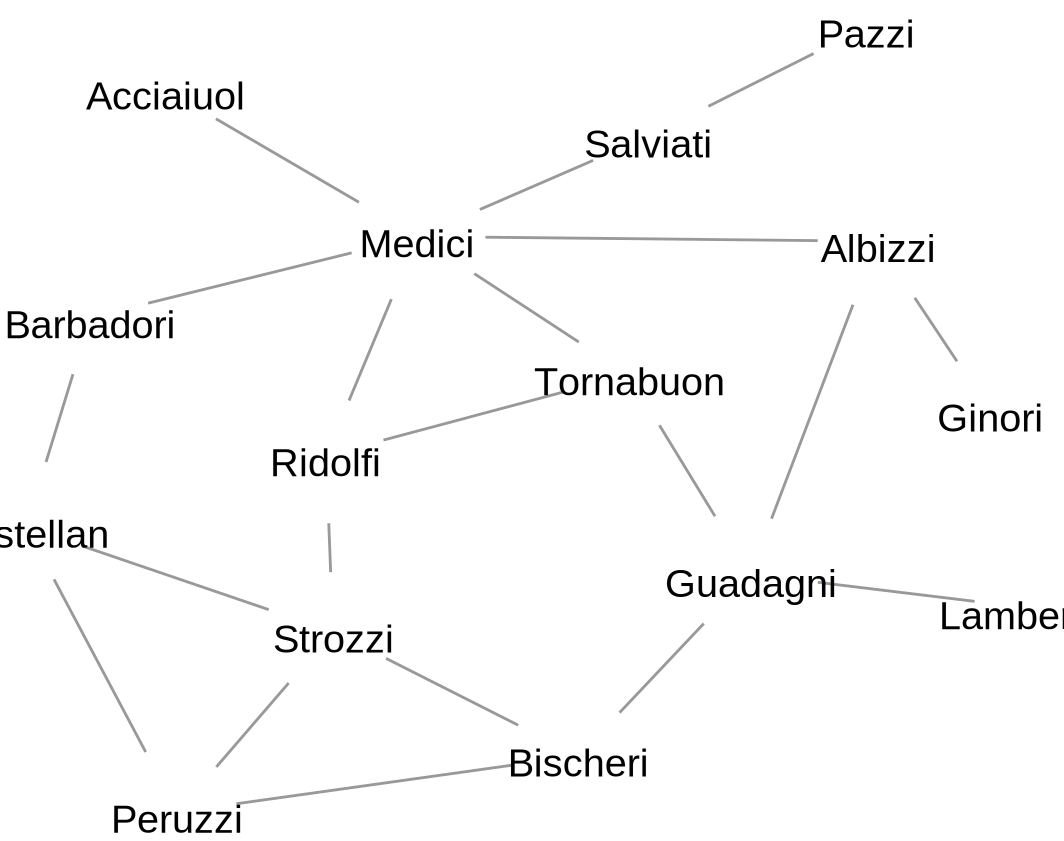
\includegraphics{images/nobility.pdf}}} 
%\end{figure}
%
%Take, for example, the Florentine nobility network~\cite{PadgettA93}, shown in
%Figure~\ref{fig:nobility}. The Medici family has a betweenness centrality of
%0.522 by itself, and the next best single family has betweenness centrality of
%0.255 (Guadagni). However, there are many pairs of individually weak families
%which can significantly improve their status by lying during the
%synchronization protocol. For example, the Tournabuon and Strozzi families may
%use the strategy we define in Section~\ref{sec:strategies} (essentially, lying
%by an additive factor of two) to improve their betweenness centrality from
%0.414 to 0.623, a multiplicative improvement of 1.5. In fact, there are many
%pairs that can make such improvements, and similar opportunities arise in other
%classic networks such as Zachary's karate club~\cite{Zachary77}. 

\subsection{NP-hardness and submodularity} \label{sec:combinatorial}

To provide a contrast with our collusion model, we present a model of
monitoring information that involves no lies. In other words, if the colluding
agents are forced to follow the synchronization and information routing 
protocols, how do we pick which nodes should collude?

\begin{problem}[$p$-Shortest Path Dominating Set] \label{prob:spds}
Given a graph $G = (V,E)$ an integer $k \geq 1$ and $p \in [0,1]$, is there a
set $S \subset V$ of size $k$ so that at least $p \binom{n}{2}$ shortest paths
pass through $S$?
\end{problem}

We abbreviate this by SPDS$(p,k)$ and say a vertex $v$ \emph{covers} a path if
it lies on the path. There are two natural optimization problems associated
with SPDS. The first, MAX-SPDS$(-,k)$, is to maximize the $p$ achieved over all
sets of size $k$. The second, MIN-SPDS$(p,-)$, minimizes $k$ while attaining a
prespecified $p$. SPDS$(p,k)$ is trivially NP-hard because SPDS$(1, k)$ is
VERTEX-COVER.
 
By a standard argument, the function $f: 2^V \to [0,1]$ mapping $S$ to the
proportion of shortest paths covered by $S$ is submodular\footnote{Recall a set
function $f:2^X \to \mathbb{R}$ is \emph{submodular} if for every $S, T \subset
X$ with $S \subset T$ and for every $x \in X \setminus T$, the marginal gain
$f(S \cup \{ x \}) - f(S) \geq f(T \cup \{ x \}) - f(T)$} and monotone.  Hence,
by a classic theorem of Nemhauser, Wolsey, and Fisher~\cite{NemhauserWF78}, the
greedy algorithm provides a $(1-1/e)$-approximation algorithm for
MAX-SPDS$(-,k)$. A slight variant of the greedy algorithm presented by
Wolsey~\cite{Wolsey82} achieves a $p$-proportion of shortest paths with a set
$S$ of size

$$ |S| = \left [ 1 + \log \max_{v \in V} f(\{ v \}) \right ] OPT
       = \left [ 1 + O(\log(n)) \right ] OPT$$

where OPT is the size of the smallest set covering a $p$-proportion of shortest
paths. 

A similar reduction from VERTEX-COVER shows that the problem of picking
colluding nodes \emph{and} a good strategy for lying is also NP-hard. Moreover,
the collusion problem is not submodular. We prove this below, and as such, we
will henceforth focus on the problem of determining the optimal strategy for a
given set of colluding agents.

\begin{proposition} \label{prop:not-submodular}

Fix $\theta(S)$ mapping subsets of vertices to optimal strategies. Define $f:
2^{V(G)} \to \mathbb{R}$ by letting $f(S) = p_{S, \theta(S)}$. Then $f$ is not
submodular. 

\end{proposition}

\begin{proof}

Let $G = K_{m,2}$ be the complete bipartite graph on parts $X,Y$ with $X = \{
p,q \}, |Y|=m$. Let $S = \{ \}, T = \{ p \}$. Then adding $q$ to $T$ captures
every path in $G$. Adding $q$ to $S$ captures only the messages sent to and
from $q$, because other messages are routed via $p$. In particular,

\begin{align*}
   f(S \cup \{ q \}) - f(S) &= 2(m+1) = O(m) \\ 
   f(T \cup \{ q \}) - f(T) &= 2 \binom{m+2}{2} - 2(m+1) = O(m^2),
\end{align*}

disproving submodularity. 
\end{proof}

There are also interesting examples of this that rely on lies in a nontrivial
way, for example when $G = C_n$ for sufficiently large $n$. In this case a
single node has little advantage, but adding a second adjacent node allows for
an interesting collusion. One of the two colluders may broadcast 1 for most
targets, and forward incoming messages to the its neighboring colluder who in
turn forwards along $C_n$ to the target. We discuss the broadcast bounds for
this case in Section~\ref{sec:unseparated}.

\subsection{A reduction from nonuniform to uniform} \label{sec:reduction}

We define decision problems for the uniform and nonuniform variants of our
model and prove that the nonuniform case reduces to the uniform case with a
small blowup.

\begin{problem}[UNIFORM-SUBSET-MONITORING]

Given a graph $G = (V,E)$ a subset $S \subset V$ and a $p \in [0,1]$, is there
an admissible strategy $\theta$ for $S$ such that in the uniform broadcast
model $p_{S, \theta} \geq p$?

\end{problem} 
 
For nonuniform lies, we analogously define NONUNIFORM-SUBSET-MONITORING.
Nonuniform lies might appear at first glance to provide a substantial increase
in power (there are many more strategies, and it seems easier to accidentally
introduce a large cycle as in Figure~\ref{fig:nonuniform-cycle}), we show that
algorithmically finding the optimal nonuniform strategy for a fixed subset is
no harder than finding the optimal uniform strategy. This justifies a detailed
study of the uniform model.

\begin{figure}[b]
\centering
\includegraphics[width=0.5\textwidth]{images/5cycle.pdf}
\caption{In this nonuniform example, $w$ is the target of a message sent from $x$. The
colluding agent $u$ broadcasts $\rho(u,w) = 1$ to $v$, and $\rho(u,w) = 7$ to
$x$. However, $u$'s lie propagates around the cycle to $y$, so that any message
sent through $y$ to $w$ would be forwarded to $v$.}
\label{fig:nonuniform-cycle}
\end{figure}

\begin{proposition} \label{prop:uniform-reduction}

NONUNIFORM-SUBSET-MONITORING reduces to UNIFORM-SUBSET-MONITORING.

\end{proposition}

\begin{proof}

Given a graph $G$, a subset $S$, and a fraction $p$ for the nonuniform model,
we produce a new graph $G'$, a subset $S'$, and a fraction $p'$ for the uniform
model as follows. For simplicity we will prove the case where $G$ is
$D$-regular. Start by setting $G' = G$. For each edge $e = (u,v)$ where $u \in
S$, subdivide $e$ in $G'$ with a new vertex $w_e$. Also for each such edge, add
$u, w_e$ to $S'$.  Finally, set 

\[ 
   p' = \frac{p\binom{|V|}{2} + \binom{|S|D}{2} + |S||V|}{\binom{|V| +
   |S|D}{2}}.
\]

Suppose there is a strategy $\theta$ for $S,G$ achieving a $p$ fraction in the
nonuniform model. We'll convert $\theta$ into a strategy $\theta'$ for $S'$.
Whenever a colluding agent $u \in S$ would broadcast $\rho$ to a neighbor $v$,
we have the agent $w_{(u,v)}$ uniformly broadcast $\rho$.  And whenever a
message goes to $w_{(u,v)}$ with some other destination, $w_{(u,v)}$ forwards
it through $u$, who in turn forwards it to the $w_{(u,v')}$ corresponding to
the same $v'$ that $u$ would forward to in the nonuniform setting. This
simulates $\theta$, and hence achieves the same $p\binom{|V|}{2}$ paths in $G$;
the formula for $p'$ simply counts the paths introduced by the new vertices
(all of which include a colluding agent). So if $p_{S,\theta} \geq p$ in $G$,
$p_{S', \theta'} \geq p'$ in $G'$.

Conversely, we can collapse any uniform strategy for $S'$ into a nonuniform one
for $S$ by contracting all the newly added edges in $G'$ and combining their
broadcasts in the obvious way. The case where $G$ is irregular is analogous,
and it's clear the appropriate $p'$ can be efficiently computed.
\end{proof}

\section{Strategies for the uniform model} \label{sec:strategies}

We now turn to a detailed study of the uniform broadcast model. In this section
we prove Theorem~\ref{thm:main}, restated below.

\begin{theorem} \label{thm:optimal-separated}

Let $G = (V,E)$ be a graph and $S \subset V$ a fixed subset of vertices such
that $d(x, y) \geq 2$ for all $x,y \in S$. Then the strategy $\rho^*$ defined
in Section~\ref{sec:separated} intercepts an optimal fraction of traffic in
$G$.

\end{theorem}

The proof consists of two parts. After defining the broadcast policy
$\rho^*$ in Section~\ref{sec:separated} and the associated forwarding
policy, we first prove in Proposition~\ref{prop:rhostar-admissible} that the
strategy is admissible, and then in Proposition~\ref{prop:rhostar-lower-bound}
that $\rho^*$ is the minimal broadcast for any admissible strategy.

\subsection{A single agent} \label{sec:single-agent}

We start by characterizing the case of a single colluding agent. This case is
useful because it forms a sort of ``base case'' for our more complicated
strategies. In this case the best strategy is simple: lie exactly two less than
your true distance to a target. This is guaranteed not to cause cycles, while
any larger lie causes a cycle of length 2. In this case broadcasts will not
change across rounds, and so we use $\rho(x,y)$ to denote the broadcast by $x$
about its distance to $y$ across all rounds.

\begin{theorem} \label{thm:single-agent}

Let $x$ be a colluding node and $t$ be a target node whose true distance in $G$
is $d(x,t) = k$. Suppose that $x$ broadcasts $\rho(x,t) = k'$. Then this
strategy is admissible and beneficial if and only if one of the following
conditions hold.

\begin{enumerate}
   \item $k' = k - 2$ and there is a neighbor $z$ of $x$ with $d(z,t) = k = k'
+ 2$.
   \item $k-2 \leq k' \leq k-1$ and there is a neighbor $z$ of $x$ with $d(z,t)
= k + 1$, and there is a shortest path from $z$ to $t$ that does not pass
through $x$ (before $x$'s lie).
\end{enumerate}

\end{theorem}

\begin{proof}

Note that $d(x,t) = k$ if and only if the closest neighbor $y$ of $x$ to $t$
has distance $d(y,t) = k-1$. The strategy for $x$ will be to route all messages
to $t$ through $y$.

For one direction, suppose one of the above conditions holds and let $z$ be a
neighbor of $x$ satisfying the desired property. Then $z$ will send messages to
$t$ through $x$, which $x$ can forward through $y$. We further claim that no
message forwarded through $y$ to $t$ will ever come back to $x$. Call $y, v_2,
v_3, \dots$ the vertices on the route taken by the sent message after passing
through $x$. The tie-breaking assumption implies $v_2 \neq x$, and it follows
that the perceived distances $\rho(v_i, t)$ along the message's path from $t$
are monotonically decreasing in $i$. This follows from the fact that $x$
broadcasts the same lie to all its neighbors. In particular, $\rho(x,t) =
\rho(v_2, t)$ and so for all $j \geq 2$, $v_j$ will always have a closer
neighbor than $x$.

For the converse, suppose the strategy is admissible and beneficial. First, $x$
cannot broadcast $\rho(x,t) < k-2$, or else $y$ (and by minimality all
neighbors of $x$) will route messages to $t$ through $x$, causing a cycle. If
$k' \geq k$, then no neighbor of $x$ would change its behavior, contradicting
beneficialness. This implies the conditions on $k'$ in (1) and (2). Moreover,
beneficialness implies $x$ has a neighbor $z$ that now forwards messages
through $x$, implying its new perceived distance is $\rho(z,t) = k' + 1$. By
the fact that $d(x,t) = k$, every other neighbor $z$ of $x$ has $k-1 \leq
d(z,t) \leq k+1$. If all neighbors have distance $k-1$ then the tie-breaking
assumption implies the strategy is not beneficial, so let $z$ be a neighbor
with $d(z,t) \geq k$.

If $d(z,t) = k$ then the shortest path from $z$ to $t$ already does not pass
through $x$ and we must choose $k' = k-2$ to change $z$'s behavior. On the
other hand, if $d(z,t) = k+1$ but has no other shortest path to $t$ except
through $x$, then lying is not beneficial. If $z$ has another
path to $t$ then setting $k' = k-1$ breaks the tie.
\end{proof}

One can simplify the above lemma by noting that setting $k' = k-2$ is always
nondetrimental, and this is the optimal nondetrimental lie. So if an agent has
incentive to lie, it may as well lie as much as possible. This proves the
following corollary.

\begin{corollary} \label{cor:single-agent}

Let $x$ be a single lying agent in $G$ in the uniform local broadcast model. An
optimal admissible strategy for a single lying agent $x$ is to broadcast
$\rho(x,t) = \max(1, d(x,t) - 2)$ for all $t \in V(G)$.

\end{corollary}

The same algorithm can be jointly and independently used by multiple colluding
agents in the uniform broadcast model. We make this rigorous with the following
proposition.

\begin{proposition} \label{prop:independent-agents}

If any set of colluding agents lie independently according to
Corollary~\ref{cor:single-agent}, then their joint strategy is admissible.

\end{proposition}

\begin{proof}

In the proof of Theorem~\ref{thm:single-agent}, we showed that a vertex $x$
lying in this way cannot produce any cycles of length 2, since it does not
alter the behavior of the neighbor through which $x$ routes messages to $t$. It
remains to show that there are no longer cycles.

Suppose to the contrary that when $s$ tries to send a message to $t$, there is
a cycle $v_1, v_2, \dots, v_m, v_{m+1} = v_1$, with $m \geq 3$. Let $i$ be the
index of a vertex on the cycle which minimizes the true distance $d(v_i, t)$.
Call this distance $a$, and note that $v_i$ is not a colluding agent (or else
it could correctly forward messages so as to break the cycle). Because there is
a cycle, $v_{i+1}$ is broadcasting $\rho(v_{i+1}, t) \leq a-2$, but $d(v_{i+1},
t) \geq a$. And since $v_{i+1}$ forwards to $v_{i+2}$, we have $\rho(v_{i+2},
t) \leq a-3$ while $d(v_{i+2}, t) \geq a$. We claim this is a contradiction: a
colluding agent lies by exactly two less than the truth, and so $v_{i+2}$
cannot be a colluding agent. But the effect of a colluding agent's lie does not
change the perceived distances of any vertex in $G$ by more than two. This
shows the claimed contradiction.
\end{proof}

\subsection{Separated agents}\label{sec:separated}

We now turn to the case of multiple colluding agents. By
Proposition~\ref{prop:uniform-reduction}, we know that allowing neighboring
colluding agents introduces the ability for nonuniform broadcasts. So we
characterize the alternative where no two colluding agents are adjacent. The
optimal strategy we define generalizes to a nontrivial admissible strategy for
the general case in Section~\ref{sec:unseparated}.

For a set $X$ and an integer $j$, define $S_X(j)$ to be the set of all
permutations of $j$ elements from $X$. In this section $C = \{ x_1, \dots, x_k
\}$ will denote the set of colluding nodes, and no two are adjacent in $G$.

\begin{definition}
The \emph{$j$-th colluding distance} between two colluding agents $x$ and $y$
is defined as

\[
   d_j(x, y)= \min_{\substack{\sigma \in S_C(j) \\ \sigma(1) = x \\ \sigma(j) =
y}}
         \sum_{i=1}^{j-1} d(\sigma(i),\sigma(i+1)).
\]

In other words, it is the length of the shortest path from $x$ to $y$ that
contains $j$ colluding nodes. Call any path minimizing this quantity a
\emph{$j$-th colluding path}. If no such path exists, call $d_j(x,y) = \infty$
by convention.  \end{definition}

We will consider $j$-th colluding paths directed from $x$ to $y$ when
appropriate. Now given a set of colluding nodes and a target vertex $t$, we
want to identify the strategy that minimizes $\rho(-,t)$ for all of our
colluders. We start by defining a candidate strategy $\rho^*$, observe that it
is admissible, and then prove it is indeed a lower bound on admissible
strategies.

\begin{definition} \label{def:colluding-distance}
Let $\rho'(x,t) = \max(d(x,t) - 2, 1)$. Let $\rho''(x, t)$ be defined as

\[
   \min_{1 \leq i,j \leq k} \left [ d_j(x,x_i)-2(j-1) + \rho'(x_i, t) \right ].
\]

Then define the strategy $\rho^*(x,t)=\min(\rho'(x,t), \rho''(x, t))$.

\end{definition}

To give some intuition, this strategy takes the minimum of
Corollary~\ref{cor:single-agent} and the best $j$-th colluding path (where the
end of that path uses Corollary~\ref{cor:single-agent} to get to $t$).

Definition~\ref{def:colluding-distance} is useful in the following scenario
depicted in Figure~\ref{fig:colluding-distance}. Suppose $(s, x_1, y_2, x_2,
\dots, y_j, x_j, t)$ is a path of length $2j + 1$, where $t$ is the target of a
message sent by $s$ and $x_i$ are colluding agents.  Then every $x_i$ may
broadcast $\rho^*(x_i, t) = 1$, and the tie breaking assumption ensures that
the honest agents will forward along the path toward $t$.

\begin{figure}[thb]
\centering
\includegraphics[width=0.5\textwidth]{images/colluding-distance.pdf}
\caption{An example of a better strategy than $\rho(x,t) = d(x,t) - 2$ when
taking into account other colluding agents. The shaded agents are colluding,
and $x$ may broadcast $\rho^*(x,t) = 1$.}
\label{fig:colluding-distance}
\end{figure}

We call $x$ \emph{proper for $t$} if it (strictly) minimizes $\rho^*(x,t)$ via
the $j$-th colluding distance for some $j \geq 2$ and \emph{improper}
otherwise, and we call a $j$-th colluding path realizing this minimization a
\emph{witness} for the properness of $x$. We define the \emph{forwarding
number} of a $j$-th colluding path to be $j$, and define the forwarding number
of a vertex $v$ to be the smallest forwarding number of any $j$-th colluding
path minimizing $\rho^*(v,t)$ starting at $v$. Note that a vertex with a
forwarding number 1 is by definition improper, and that all of these
definitions depend on the choice of $t$.

The forwarding policy is as follows. Improper colluding nodes forward as in
Corollary~\ref{cor:single-agent}. Proper colluding agents pick a $j$-th
colluding path which minimizes their broadcast, breaking ties by minimizing
forwarding number, and deterministically forward along that path. We now prove
that $\rho^*$ is an admissible strategy under worst-case tie breaking
assumptions. First we prove that $j$-th colluding paths can be extended in a
nice way.

\begin{proposition} \label{prop:inductive-path}

Let $x,y$ be colluding vertices in $G$. Then $\rho^*(x,t) \leq d(x,y) - 2 +
\rho^*(y,t)$.

\end{proposition}

\begin{proof}

If $y$ is improper, then $\rho^*(x,t)$ has a 2-th colluding path and trivially
$\rho^*(x,t) \leq d(x,y) - 2 + \rho'(y,t)$ so we are done.

So suppose $y$ is proper with forwarding number $j$. By definition, there is a
$y'$ such that $\rho^*(y,t) = d_j(y,y') - 2(j-1) + \rho'(y',t)$. Call the
witness path $\sigma$. Then there is a corresponding path $\sigma'$ for $x$
constructed by prepending a path from $x$ to $y$ to $\sigma$. This path is some
$j'$-th colluding path for $j' > j$ whose cost is an upper bound on
$d_{j'}(x,y')$.  Hence,

\begin{align*}
   \rho^*(x,t) &\leq d_{j'-j}(x,y) - 2(j' - j) + d_j(y,y') - 2(j-1) +
\rho'(y',t) \\
               &\leq d(x,y) - 2 + \rho^*(y,t),
\end{align*}

as desired.
\end{proof}

In fact, if $x$ is proper, $\rho^*(x,t)$ is minimized by computing $d(x,y) - 2
+ \rho^*(y,t)$ for some colluding agent $y$. It will have the property that
there is a path from $x$ to $y$ that passes through no other colluding agents.
Proposition~\ref{prop:inductive-path} trivially extends to non-colluding agents
$y$, giving the following corollary. Note here we use $\rho$ to denote the
broadcast (honest or lie) of any agent.

\begin{corollary} \label{cor:rhostar-bound}

If all colluding agents are following $\rho^*$, then for all $x \in C, y \in
V(G)$, $\rho^*(x,t) \leq d(x,y) - 2 + \rho(y,t)$.

\end{corollary}

Another simple consequence of Proposition~\ref{prop:inductive-path} is that the
forwarding number decreases along minimal $j$-th colluding paths.

\begin{proposition} \label{prop:inductive-forwarding-number}

Suppose $x$ is a proper colluding agent with respect to $\rho^*(x,t)$, that $x$
has forwarding number $j$, and that $\sigma$ is a witnessing $j$-th colluding
path. Let $x'$ be the first colluding agent on $\sigma$ after $x$. Then $x'$
has forwarding number $j-1$.  

\end{proposition}

\begin{proof}

The same technique from the proof of Proposition~\ref{prop:inductive-path}
shows that whatever the forwarding number of $x'$ is, we can prepend a path from
$x$ to $x'$ to get a path with forwarding number $j+1$.
\end{proof}

In particular, the $i$-th visited colluding agent on a witness for
$\rho^*(x,t)$ of forwarding number $j$ has forwarding number exactly $j - i$,
and the end of the path is an improper colluding agent.

At this point one might expect some sensible extension of the pair of
(forwarding number, broadcasted distance) to honest agents would produce a
potential function that is monotonically decreasing along the message path and
zero at the target. Indeed, a version of this is true when the colluding agents
are separated by distance at least three, with ready counterexamples for
distance two. Still, we present a different argument that $\rho^*$ is also
admissible when the agents are distance two apart.
 
\begin{proposition} \label{prop:rhostar-admissible}

Let $C = \{ x_1, \dots, x_k \}$, and suppose that $d(x_i, x_j) \geq 2$ for all
$x_i, x_j \in C$. Then $\rho^*$ is admissible.

\end{proposition}

\begin{proof}

Let $s,t$ be arbitrary vertices in $G$, and let $L = (y_1, y_2, ..., y_m)$ be a
cycle in the path of a message sent from $s$ to $t$ (possibly infinite and
repeating). If the $y_i$ are all honest or improper agents we are reduced to
the case of Proposition~\ref{prop:independent-agents}. So some of the $y_i$
must be proper colluding agents. 

Without loss of generality suppose $y_1$ is a colluding agent, and let $p$ be
the minimal colluding path it forwards along, extended to the target $t$.  Let
$y_j$ be the last vertex on $L$ that is not also on $p$. The claim is that
$y_j$'s decision to forward along $L$ or $p$ is a tie break. This proves the
proposition because the tie-breaking assumption would force $y_j$ to break the
cycle.

Let $z$ be the vertex following $y_j$ on $p$, and suppose to the contrary
$\rho(y_{j+1}, t) < \rho(z,t)$. Let $x$ be the last colluding agent on $p$
before $y_j$. Let $x'$ be the first colluding agent on $p$ after $y_j$ (it may
be the case that $x' = z$). If $x$ is the last colluding agent on $p$, then let
$x'=t$ and the proof proceeds similarly. First we expand $\rho^*(x,t) + 2$
along $p$.

\begin{align*}
   \rho^*(x,t) + 2 &= d(x,x') + \rho(x',t) \\  
                   &= d(x,y_j) + 1 + d(z,x') + \rho(x',t) \\
                   &= d(x,y_j) + 1 + \rho(z,t)
\end{align*}

We now bound $\rho^*(x,t) + 2$ along $L$ using
Corollary~\ref{cor:rhostar-bound}. 

\begin{align*}
   \rho^*(x,t) + 2 &\leq d(x, y_j) + 1 + \rho(y_{j+1}, t) \\  
                   &< d(x, y_j) + 1 + \rho(z,t) \\ 
                   &= \rho^*(x,t) + 2
\end{align*}

A contradiction.
\end{proof}

Next we prove that in the separated setting $\rho^*$ is a lower bound on
admissible broadcasts. 

\begin{proposition} \label{prop:rhostar-lower-bound}

Any colluding agent broadcasting $\rho(x,t) < \rho^*(x,t)$ necessarily causes a
cycle.

\end{proposition}

\begin{proof}

Suppose to the contrary some colluding agent $x$ broadcasts $\rho(x,t) <
\rho^*(x,t)$. We will show that all neighbors of $x$ forward to $t$ through
$x$, necessarily causing cycle of length 2. Fix any neighbor $z$ and suppose to
the contrary that there is a neighbor $y \neq x$ of $z$ with $\rho(y,t) \leq
\rho(x,t)$. But then $\rho(x,t) < \rho^*(x,t) \leq d(x,y) - 2 + \rho(y,t) =
\rho(y,t)$ by Corollary~\ref{cor:rhostar-bound}, a contradiction.
\end{proof}

This completes the proof of Theorem~\ref{thm:optimal-separated}.

Finally, $\rho^*$ can be efficiently computed. The idea is to grow a search
tree of colluding agents from $t$, noting that the value of $\rho^*$ for a
new vertex is minimized by using some set of previously visited nodes. More
rigorously, for each target $t \in V(G)$ run the following procedure. Set $S =
\{ t \}$.  While $C \not \subset S$ is missing some colluding agent, take any
colluding agent with minimal distance to $S$ (true distance in $G$), and
calculate the value of $\rho^*(x,t)$ as $\rho^*(x,t) = \min_{y \in S} d(x,y) -
2 + \rho(y,t)$. Then add $x$ to $S$ and continue. Using the same arguments used
previously, it is easy to see that this will compute the correct value of
$\rho^*$ for every colluding agent and every target. Moreover, one can
construct the corresponding $j$-th colluding paths during this process. We
provide some example simulations of using this strategy on synthetic and
real-world networks in Section~\ref{sec:simulations}.

\subsection{Adjacent colluding agents} \label{sec:unseparated}

In this section we extend the strategy from Section~\ref{sec:separated} to the
setting where colluding agents may be adjacent in the network. We show this
generalization is not optimal, and instead give a family of strategies, one of
which must be optimal.

Before we state our theorems, we describe another connection between the
uniform and non-uniform models from Section~\ref{sec:models}, that we can
transform an instance of the uniform model into an instance of the nonuniform
model in which colluding agents are separated.  Specifically, one can take the
quotient $G/\sim$ of the graph $G$ by declaring two colluding agents to be
equivalent if they are in the same connected component in the induced subgraph
of colluding agents. Uniform strategies translate into nonuniform ones as
follows. If $A$ is a connected component of colluding agents collapsed to $v_A$
with neighbors $\partial_G A = N_{G/\sim}(v_A)$, then the broadcast for $v_A$
to a neighbor $w$ is the minimum over all such broadcasts from vertices in $A$.
Whenever the forwarding policy in $G$ had the form: ``receive from some $w$
with target $t$ at $x \in A$, forward through $A$ to some final node $y \in A$,
who forwards to $w'$,'' the forwarding policy in $G/\sim$ is: ``Forward
messages from $w$ with target $t$ to $w'$.''

Moreover, the concepts of forwarding number and colluding paths defined in
Section~\ref{sec:separated} for separated agents in the uniform model have
analogous definitions in the nonuniform model.  So when we say that a component
$A \subset V(G)$ has a minimal $j$-th colluding path, the $j$ refers to the
path in the quotient graph, which lifts to a path in $G$ (one of many, and
possibly involving many more than $j$ colluders).  The strategy of forwarding
along a minimal colluding path lifts from the quotient graph to a strategy that
forwards along paths between connected components.

With this understanding, the main strategy can be sketched as follows. Each
connected component of colluding agents $A \subset C$ determines a minimal
$j$-th colluding path $p_t$ for each target $t \in V(G)$ using the algorithm
from Section~\ref{sec:separated}. Pick any $x \in A$ which is adjacent to the
first honest vertex $w$ on $p_t$, call this the \emph{$t$-exit node} for $A$,
and have $x$ broadcast $\rho(x,t) = \rho(w,t) - 1$ as usual. If every
non-$t$-exit node in $A$ broadcasts so that the message never returns to $A$,
then the proof of Proposition~\ref{prop:rhostar-admissible} generalizes to
prove no cycles occur for this strategy. 

We now describe bounds on the minimality of such broadcasts. For $A \subset
V(G)$, denote by $d_{G - A}(x,y)$ the distance from $x$ to $y$ in the subgraph
induced by $V(G) - A$. When $A = \{ a \}$ is a single node we abuse notation
and write $d_{G-a}$. We further write $\rho_{G-A}$ to denote the
perceived/broadcast distances when $A$ is removed. Note these values change for
honest agents when paths are eliminated, but not for colluding agents. 

As a simple illustrative first case, suppose there are exactly two colluding
agents $x,y$ and they are adjacent. Let $t \in V(G) - \{ x,y \}$. If $y$
forwards a message to $x$, who in turn forwards to $t$ through $w \neq y$, then
in order to prevent the message cycling back though $y$, we require
$d_{G-x}(w,y) + \rho(y,t) \geq d(w,t)$, which rearranges to give a condition on
$y$'s broadcast. If $d_{G-x}(w,y) = \infty$ this is interpreted as no
restriction, and $\rho(y,t)$ may be 1.

For a connected component $A$ and target $t$, a similar bound is imposed on
every node in $A$ which is not the $t$-exit node. We state it as a theorem.

\begin{theorem}\label{thm:generalization}

Let $G$ be a graph, $C \subset V(G)$ be a subset of colluding agents whose
induced subgraph has components $C_1 \cup \dots \cup C_s$. For each component
$C_i$ and target $t$, pick a $t$-exit node $v_{i,t} \in C_i$, who behaves as
described above, and have every $x \in C_i$ forward messages with target $t$ to
$v_{i,t}$. Call $w_{i,t}$ the node that $v_{i,t}$ forwards to. Pick any
broadcast of the non-exit nodes $x \in C_i$ such that for all $j$ with $C_j$
having no larger forwarding number,

\[ 
    \rho(x,t) \geq \rho(w_{j,t},t) - d_{G-(C_j - \{ x \} )}(w_{j,t}, x),
\]

setting $\rho(x,t) = 1$ if all of the above bounds are nonpositive or
$-\infty$. 

This strategy is admissible.

\end{theorem}

\begin{proof}

As discussed above, it suffices to show that a message for $t$ forwarded
through $C_i$ to the $t$-exit node $v_{i,t}$ never returns to $A$. Suppose to
the contrary the message follows some path $p$ hitting $x \in C_i$. Without
loss of generality, $x \neq v_{i,t}$ is the first to receive the message. Now
$\rho(w_{i,t}, x) \geq d_{G-(C_i - \{ x \})}(w_{i,t}, x)$, and so by assumption
(that $x$ gets the message), they are equal and $w_{i,t}$ is in a tie-break
situation.
\end{proof}

This strategy is not optimal. Figure~\ref{fig:forwarding-ctex} gives a
counterexample, in which the central issue is that two components which are
tied for minimal forwarding number could improve their joint strategy by having
one component forward through the other. In contrast to the separated case, a
different choice of forwarding policy implies different broadcasts for the
nodes. Indeed, if $X$ is the space of all strategies induced by all possible
forwarding configurations and the implied broadcasts from
Theorem~\ref{thm:generalization}, it is easy to see that an optimal strategy is
a member of $X$.  Still, it is unclear whether it is NP-hard to pick the
optimal forwarding policy.


\begin{figure}[h]
\floatbox[{\capbeside\thisfloatsetup{capbesideposition={right,center},
capbesidewidth=9cm}}]{figure}[\FBwidth]
{\caption{A counterexample to the optimality of our strategy in the setting
where agents can be adjacent. Shaded nodes are colluding. If the component with
$z,y$ is processed first then our algorithm correctly chooses the $w,x$
component to have forwarding number 2 (with $x$ broadcasting 1), capturing all
traffic from $a,b$ to $t$.  On the other hand if $w,x$ is processed first the
result will miss traffic from $a,b$.} \label{fig:forwarding-ctex}}
{\scalebox{1.5}{
\includegraphics{images/forwarding-ctex.pdf}}} \end{figure}


\section{Simulations} \label{sec:simulations}
 
We simulated the protocols described in this paper on four
networks.\footnote{The code used to run the experiments is available at
\url{https://github.com/j2kun/information-monitoring-simulations}.} The first
is an Erd\"os R\'enyi random graph $G(n, p)$ where $n = 1000, p = 4/1000$. The
second is a preferential attachment model~\cite{BarabasiA99} with 100 nodes.
The third is a Watts-Strogatz model~\cite{WattsS98} with $n=1000$, degree
$k$=10, and edge-rewiring probability $\beta=0.04$. The fourth is a snapshot of
the Autonomous Systems subgraph of the United States, which has 9,296 nodes and
17,544 edges. The AS graph comes from the website of Newman~\cite{Newman06}.
For both, we ran two tests to inspect the potential advantage of the $\rho^*$
strategy of Section~\ref{sec:separated} over the strategy in which all agents
act independently according to $\rho(x,t) = d(x,t) - 2$. We also compared the
success of the best strategy for a randomly chosen subset of nodes versus nodes
of high degree.

As expected large degree nodes tend to be better colluders than randomly chosen
nodes. Regardless, the benefit of colluding is clear even for randomly chosen
nodes. In fact for the US AS network, if we compromise only 18 random nodes
(roughly 0.2\%) we can monitor an expected 10\% of the entire network's
traffic. For smaller percentages, the randomly selected colluding nodes capture
more traffic in the US AS network than in the synthetic models. However, for
larger percentages the amount of captured traffic in the US AS network levels
off quite dramatically, revealing additional topological structure in the US AS
network that is not present in the synthetic models. It is also interesting to
note the relatively small difference between the two strategies in the US AS
graph, implying that in this setting collusion does not provide a
quantitatively large improvement over a simpler strategy. We stress that since
the $\rho^*$ strategy (as defined in Section~\ref{sec:separated}) may not be
optimal when there are adjacent colluding nodes, the plots are lower bounds for
the amount of traffic captured by the optimal strategy with a given percentage
of colluding nodes. For uniform broadcasts and small random colluding sets, our
estimates are fairly accurate because with high probability none of the
colluders are adjacent. On the other hand, for nonuniform broadcasts the
optimal strategy for 18 random nodes could very well capture more than 10\% of
the US AS traffic.

\begin{figure}[htbp]
\centering
\subfigure{
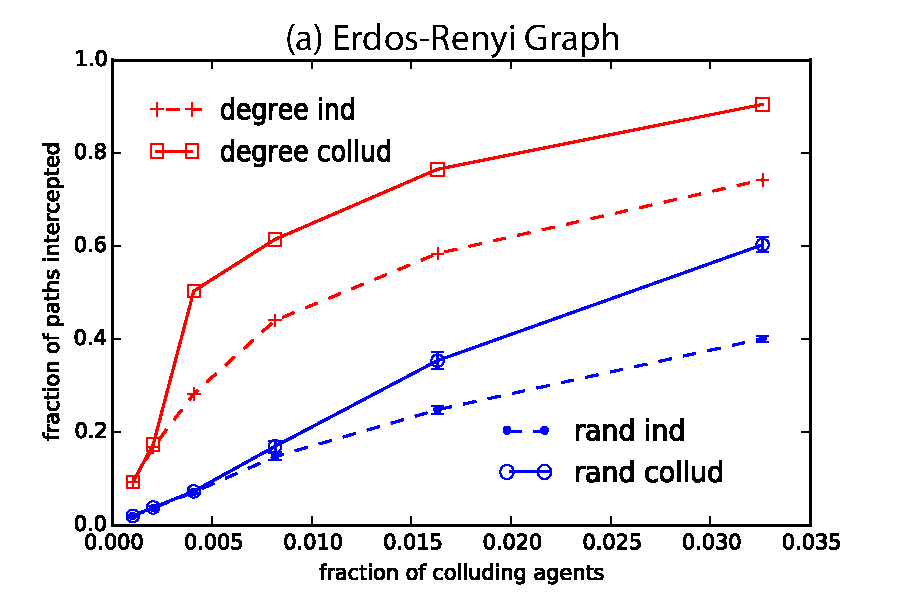
\includegraphics[width=0.45\textwidth]{images/erdosrenyi.pdf}
}
\quad
\subfigure{
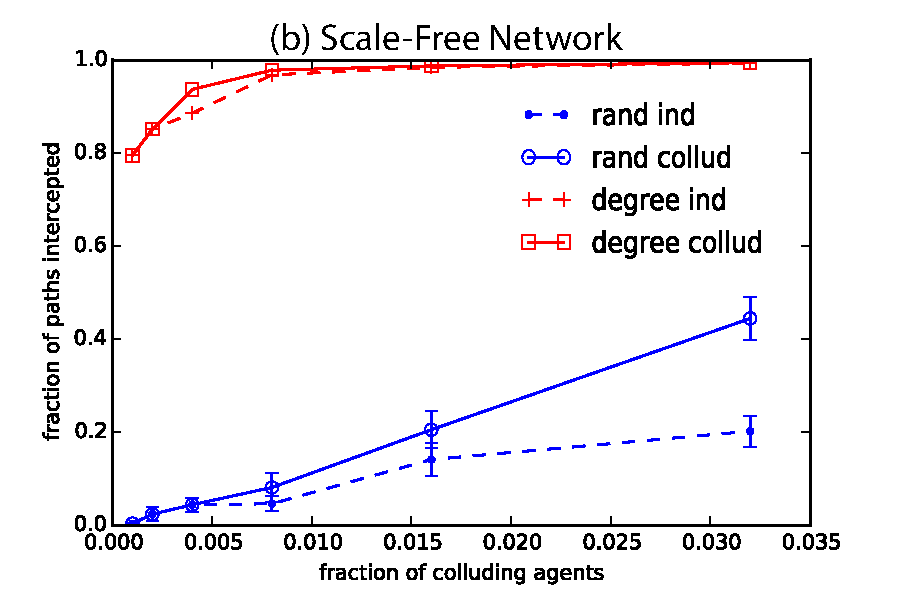
\includegraphics[width=0.45\textwidth]{images/barabasi.pdf}
}
\\
\subfigure{
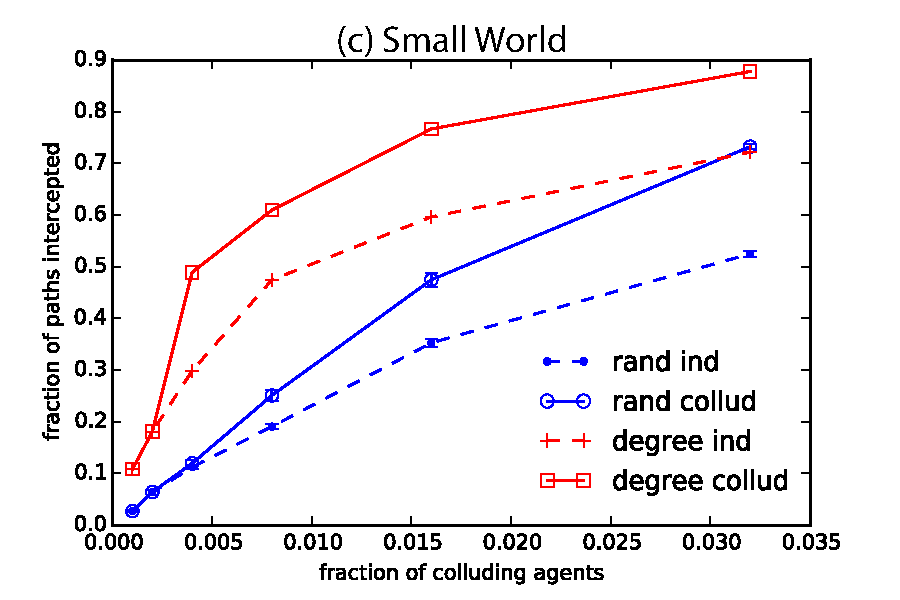
\includegraphics[width=0.45\textwidth]{images/watts.pdf}
}
\quad
\subfigure{
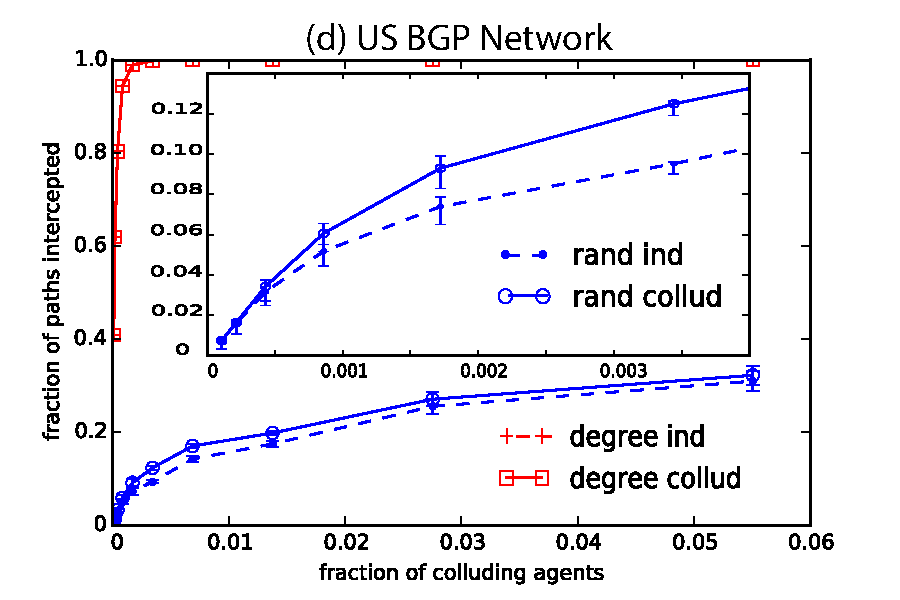
\includegraphics[width=0.45\textwidth]{images/US.pdf}
}
\caption{Fraction of paths intercepted by a varying number of colluding agents
on a Erd\"os-R\'enyi random graph (top left), a preferential attachment graph
(top right), a Watts-Strogatz model (bottom left), and the US AS network
(bottom right). Blue curves represent subsets of colluding agents chosen
uniformly at random, while red curves represent subsets chosen by largest
degree. Dashed curves indicate the strategy where each agent independently lies
by an additive factor of two, while solid curves indicate the optimal separated
strategy of Section~\ref{sec:separated}. The inset graph for the AS network
magnifies the leftmost portion of the blue curve.}

\label{fig:erdos-renyi}
\end{figure}


\section{Discussion and open problems} \label{sec:conclusion}

In this paper we introduced and related two variants of a model of
information monitoring in networks, one for uniform broadcasts and one for
non-uniform broadcasts. We characterized the optimal strategy for the uniform
setting in which no two colluding agents are adjacent, and provided a family of
strategies for the general case. We simulated the impact of the optimal
strategy in the uniform broadcasting model on an assortment of graphs and found
that in expectation for the US Autonomous Systems network, randomly selecting
.02\% of the nodes to act as colluding agents captured 10\% of the entire
network traffic.  

There are a few directions for future work. The most natural question is
whether one can efficiently characterize the general case of adjacent agents,
or whether deciding the appropriate forwarding mechanism is NP-hard. In either
case, another open direction is to provide approximation algorithms when the
optimal subset of colluding agents is unknown. This is likely to correlate with
betweenness centrality to begin with, but more interesting is to find the
subset of agents with the largest \emph{relative} improvement.

\section{Thanks} 

We thank everyone involved in the 2014 AMS Network Science Mathematical
Research Community for inspiration and many helpful comments, especially the
organizers Aaron Clauset, David Kempe, and Mason Porter. We also thank Lev
Reyzin for his helpful comments.


\bibliography{main}

\end{document}
